\documentclass[12pt]{extarticle}

%------ paramètres généraux et commandes prédéfinies
%%%% Pour avoir les accents et autre caractère français
\usepackage[french]{babel}
\usepackage[T1]{fontenc}
\usepackage[utf8]{inputenc}

%%%% Paquets utilisé
\usepackage{ifthen} % pour programmer avec des boucle et des conditions
%% Images/dessin
\usepackage{subcaption} % pour les légendes des figures
\usepackage{graphicx} % pour insérer des images
\usepackage[european, straightvoltages, RPvoltages]{circuitikz} % pour dessiner des circuits électrique
\usepackage{pdfpages} % pour inclure des fichiers pdf
\usepackage{wrapfig} % pour entourer les images par du texte 
\usepackage{chemfig} % pour dessiner des formules chimiques
\usepackage{fontawesome} % pour dessiner de jolies icônes
%% Mise en page
\usepackage{geometry} % définition des marges
\usepackage{dashundergaps} % pour avoir générer des textes à compléter
\usepackage{fancyhdr} % pour faire des en-tête
\usepackage[many]{tcolorbox} % pour faire de jolie boîtes colorée
\usepackage{enumitem} % pour pouvoir définir des listes personnalisées
\usepackage{hyperref} % pour insérer des liens
\usepackage{multicol} % pour avoir plusieurs colonnes côte-à-côte
\usepackage{listings} % pour insérer du code
%% Tableau
\usepackage{tabularray} % pour avoir de meilleurs tableaux
%% Math
\usepackage{amsmath} % symboles mathématiques
\usepackage{amssymb} % symboles mathématiques en gras
\usepackage{wasysym} % pour avoir des symbole d'intégrale
\usepackage{accents} % pour les notations mathématiques avec une barre
\usepackage{physics} % pour les dérivées, les bra, les kets, etc.
\usepackage{esvect} % pour faire de jolis vecteurs
\usepackage{siunitx} % pour avoir de jolie grandeurs avec des unités 
%% Décommenter pour avoir une police spéciale dysléxie (doit être compilé en XeTeX)
% \usepackage{fontspec}
% \setmainfont{OpenDyslexic}


%%%% Réglages de la taille des indentations et des sauts de paragraphes
\setlength{\parskip}{0cm}
\setlength{\parindent}{0cm}
\renewcommand{\baselinestretch}{1}
% réglage du niveau (sous-section) ou s'arrête la table des matières
\setcounter{tocdepth}{2}


%%%% Réglage de la géométrie des pages
\geometry{
  a4paper, % format
  left=1.3cm, right=1.3cm, % marge horizontale
  top=2.2cm, bottom=2.3cm % marge verticale
}


%%%% Réglage de chemfig
\setchemfig{
  atom sep=26pt,
  bond style={line width=1pt},
  angle increment=30
}


%%% Apparence (couleur) des liens
\hypersetup{
  colorlinks=true,
  linkcolor=black, % lien type table des matière
  citecolor=black, % citation
  filecolor=black, 
  urlcolor=blue!90!black % lien internet
}


%%%% Réglage de tikz (flèche et caractères)
\usetikzlibrary{babel}
\tikzset{>=latex}


%%%% Réglage des en-tête
\renewcommand{\headrulewidth}{0.4pt}
\setlength{\headheight}{22.50113pt}


%%%% Réglage de dashundergaps pour avoir des points et pas de numération
\dashundergapssetup{
  gap-numbers = false,
  gap-format = dot,
  gap-widen,
  gap-extend-percent
}


%%%% Réglage de siunit
\sisetup{
  locale = FR, % français
	 group-minimum-digits = 4, % groupage des chiffres par millier
  inter-unit-product = \ensuremath { { } \cdot { } } % point médian entre les unités
}
\AtBeginDocument{\RenewCommandCopy\qty\SI} % Pour "écraser" la commande \qty du package physics
% \geometry{a4paper, landscape} % format paysage
% \geometry{a5paper, left=1cm, right=1cm, top=0.8cm, bottom=2cm} % format A5
% \modeCorrection % correction (décommenté)
\renewcommand{\etablissement}{Lycée Jean Moulin} % pour l'en-tête

% 60, 50, 45, 40, 30: 0.866, 0.766, 0.707, 0.643, 0.5
\NewDocumentCommand{\chemPolygone}{O{} r()}{
  \pgfkeys{/chemPoly, defaut, #1}
  \node [
    regular polygon, fill = \chemCouleur,
    regular polygon sides = \chemBords, 
    inner sep = \fpeval{\chemAtomSep * \chemBords * 0.103} pt,
    rotate = \chemRotation,
  ] at (#2) {};
}
%
\NewDocumentCommand{\chemPentagoneHaw}{O{} r()}{
  \pgfkeys{/chemPoly, defaut, couleur = orange-150, #1}
  \coordinate (A) at (#2);
  \fill [fill = \chemCouleur] 
    ($(A) + (0pt, 0pt)$) --
    ($(A) + 1.4*(20pt, 12pt)$) --
    ($(A) + 1.4*(40pt, 0pt)$) --
    ($(A) + 1.4*(30pt, -16pt)$) --
    ($(A) + 1.4*(9pt, -16pt)$) --
    cycle;
}
%
\NewDocumentCommand{\chemHexagoneHaw}{O{} r()}{
  \pgfkeys{/chemPoly, defaut, couleur = green-200, #1}
  \coordinate (A) at (#2);
  \fill [fill = \chemCouleur] 
    ($(A) + (0pt, -0.2pt)$) --
    ($(A) + (14pt, -16.5pt)$) --
    ($(A) + (40.3pt, -16.5pt)$) --
    ($(A) + (54.6pt, -0.5pt)$) --
    ($(A) + (38.8pt, 14.4pt)$) --
    ($(A) + (15.4pt, 14.4pt)$) --
    cycle;
}

%------ doc
\begin{document}
  \begin{tikzpicture}
    \node (base) at (0,0) {};
    \chemCarboxyle (-140pt, 14pt)
    \chemAmine (-92pt, 18pt)
    \chemAmide (78pt, 10pt)
    \node at (base) {
      \chemfig{!\alanine} $+$
      \chemfig{[:30]H_2N !\cysteineB OH} \reaction
      \chemfig{[:-30] H_2N !\alanineH !\HN !\cysteineB OH}
    };
  \end{tikzpicture}
  
  \begin{tikzpicture}
    \node (base) at (0,0) {};
    \chemAmide (-32pt,4pt);
    \node at (base) {\chemfig{[:-30] H_2N !\alanineH !\HN !\cysteineB OH}};
  \end{tikzpicture}
  %------ Commun
  % \includepdf[pages=26]{commun/papier_millimetre.pdf}
  % \newpage
\pasDePagination
\begin{center}
  \image{0.3}{images/chimie/protocoles/dissolution0001}
  \image{0.3}{images/chimie/protocoles/dissolution0006}
  \image{0.3}{images/chimie/protocoles/dissolution0003} \\[2pt]
  \image{0.3}{images/chimie/protocoles/dissolution0005}
  \image{0.3}{images/chimie/protocoles/dissolution0004}
  \image{0.3}{images/chimie/protocoles/dissolution0002}
  \\[16pt]
  \image{0.3}{images/chimie/protocoles/dissolution0001}
  \image{0.3}{images/chimie/protocoles/dissolution0006}
  \image{0.3}{images/chimie/protocoles/dissolution0003} \\[2pt]
  \image{0.3}{images/chimie/protocoles/dissolution0005}
  \image{0.3}{images/chimie/protocoles/dissolution0004}
  \image{0.3}{images/chimie/protocoles/dissolution0002}
\end{center}
  % \pasDePagination

\titre{Règles de sécurités en chimie}

\large

\important{Les 4 règles de bases :}
\begin{enumeration}
  \item Ne pas manger.
  \item Ne pas boire.
  \item Ne pas sentir.
  \item Ne pas toucher.
\end{enumeration}
Sauf indication du contraire.


\important{Pictogrammes de danger :}
\newcommand{\imagePicto}[1]{\image{0.18}{images/securite/picto_#1}}
\begin{center}
  \imagePicto{corrosif}
  \imagePicto{environnement}
  \imagePicto{toxique}
  \imagePicto{nocif}
  \imagePicto{reprotoxique}
  \imagePicto{combustible}
  \imagePicto{comburant}
  \imagePicto{explosif}
  \imagePicto{gaz_pression}
\end{center}


\titre[couleurSec]{Port de la blouse, des gants et des lunettes de protection obligatoire en travaux pratiques si demandé !}
\begin{center}
  \image{0.6}{images/exterieures/securite/picto_gant_blouse_lunette}
\end{center}

% \normalsize
% \textbf{Signature élève :}
  % \newpage
\pasDePagination

%%%%
\titre{Règles de vie en classe}

\large

\begin{listePoints}
  \item \important{Le règlement intérieur s'applique en classe.}
  \item Pas de prise de parole sans autorisation.
  \item Pas de déplacement sans autorisation.
  \item Téléphone silencieux et posés sur la table du professeur.
  \item Pas de retards acceptés passé 5 minutes.
  \item Les documents du chapitre en cours doivent \important{tous} être amenés.
\end{listePoints}

\begin{center}
  \important{Objectif : avoir un cadre de travail serein et agréable.}
\end{center}

\vspace*{-0.2cm}
\ligne

%%%
\titre{Règles d'évaluation}


\important{Les devoirs sur table}

\begin{listePoints}
  \item 1 ou 2 devoirs sur table par trimestre.
  \item \important{Date et sujet communiqués une ou deux semaines en avance.}
  \item Coefficient 3.
\end{listePoints}


\important{Les travaux pratiques}

\begin{listePoints}
  \item Évaluation des compte-rendus.
  \item Évaluation de certaines activités réalisées en classe.
  \item Évaluation de la maîtrise des gestes expérimentaux.
  \item Coefficient 2.
\end{listePoints}


\important{La progression}

\begin{listePoints}
  \item Évaluation variable (classeur, DM, interrogation).
  \item Coefficient 0,5 ou 1.
\end{listePoints}

% \bigskip
% \normalsize
% \important{Exemple :} Avec $8/20$, $9/20$, $11/20$ en devoir sur table et $10/20$ en travaux pratiques, un ou une élève assidue ($> 15/20$ en progression), s'assure une moyenne supérieure à $10/20$ (contre $9,\!5/10$ sans la progression).

% \bigskip
% \normalsize
% \important{Signature élève :}
  % \titre{Progression annuelle première ST2S}

\important{\premStssChim} \\
\important{\premStssVisi} \\ 
\important{\premStssRedo} \\ 
\important{\premStssLumi} \\ 
\important{\premStssStru} \\ 
\important{\premStssBiom} \\
\important{\premStssRout} \\
\important{\premStssAlim} \\
\important{\premStssElec} \\
\important{\premStssPres} \\
\important{\premStssSono} \\

\titre{Progression annuelle terminale ST2S}

\important{\termStssOrga} \\
\important{\termStssAlim} \\
\important{\termStssImag} \\
\important{\termStssBiom} \\
\important{\termStssMedi} \\
\important{\termStssEnvi} \\
\important{\termStssDosa} \\
\important{\termStssRout} \\
\important{\termStssCosm} \\
  % %\small

%%%% Quelques liens utiles
{\large \important{Quelques liens utiles en classe}}
\bigskip

\qrcodeCote[1]{https://nosgestesclimat.fr/tutoriel}
Nos gestes climats.
\\[22pt]

\qrcodeCote[1]{https://www.youtube.com/watch?v=OrT6vTS47f4}
Vidéos sur les VELI (pour parler du réchauffement climatique)
\\[22pt]

\qrcodeCote[1]{https://bsky.app/profile/laydgeur.bsky.social/post/3lwhxcsfeus2y}
Thread sur bsky sur l'adaptation des villes aux vagues de chaleurs

\qrcodeCote[1]{https://www.youtube.com/watch?v=z_zSd4GhOUo}
Présentation d'une étude sur la formation d'ubiquinone par des protéines dans les bactéries et de leur évolution, CNRS
\\[8pt]

\qrcodeCote[1]{https://www.youtube.com/watch?v=TEl4jeETVmg}
Présentation de la mole, avec des ordres de grandeurs, en anglais.
\\[22pt]


%%%% Lumière
\qrcodeCote[1]{https://www.youtube.com/watch?v=eaibXuVXo5s}
Vidéo de scienceclic sur les ondes électromagnétiques, complet et visuel, mais très rapide...
\\[22pt]

\qrcodeCote[1]{https://www.youtube.com/watch?v=FvbNrwjIrNU}
Présentation de la perception des couleurs chez les humains, science étonnante.
\\[22pt]

\qrcodeCote[1]{https://www.youtube.com/watch?v=w7y-1eY0mcE}
Présentation des ondes électromagnétique, et de leur utilisation dans le domaine radio, CNRS.
\\[8pt]

\qrcodeCote[1]{https://fr.science-questions.org/experiences/65/Faire_un_mirage_artificiel/?comments_page=2}
Réalisation d'un "mirage artificiel" avec un laser et une solution d'eau sucrée hétérogène.
\\[22pt]


%%%% Nucléaire
\qrcodeCote[1]{https://youtu.be/pFgTPZpjiqs?t=15}
Schématisation du fonctionnement d'une centrale nucléaire, ENGIE.
\\[22pt]

\qrcodeCote[1]{https://www.youtube.com/watch?v=ScP-uPIEpl8}
Présentation détaillée du fonctionnement d'une centrale nucléaire, le réveilleur.
\\[22pt]

\qrcodeCote[1]{https://www.youtube.com/watch?v=1MUcizMqVAc}
Présentation de la différence entre fission et fusion, science étonnante.
\\[22pt]


%%%% Son
\qrcodeCote[1]{https://www.youtube.com/watch?v=Q58ns2rLXx8}
Présentation du son, c'est pas sorcier.
\\[22pt]

\qrcodeCote[1]{https://www.youtube.com/watch?v=8YGQmV3NxMI}
Vibration d'une corde de guitare filmée avec la bonne fréquence.
\\[22pt]

% https://www.syndicalistes.org/syndiquer-en-zone-rurale
  % \pasDePagination
\begin{tblr}{
  colspec = {X[c] Q[c, 0.2\linewidth] Q[c, 0.2\linewidth] Q[c, 0.2\linewidth] Q[c, 0.2\linewidth]},
}
  Hydroxyle & 
  \chemfig{!\vide{} H-C !\HH -OH} &
  \chemfig{H-C !\HH -C !\HH -OH} &
  \chemfig{H_3C -CH_2 -CH_2 -OH} &
  \chemfig{-[:30] !\cbh !\cb OH} \\
  Carboxyle & 
  \chemfig{!\vide{:-30} H-[:30] C !\carboxyle} & 
  \chemfig{H_2 C-CH-C !\carboxyleDev} &
  \chemfig{-[:30] !\cb !\carboxyle} &
  \chemfig{-[:30] !\cbh !\carboxyle} \\
  Carbonyle &
  \chemfig{!\vide{:-30} H-[:30] C !\carbonyle H} &
  \chemfig{H_2 C-CH-C !\carbonyleDev H} &
  \chemfig{-[:30] !\cb !\carbonyle H} &
  \chemfig{-[:30] !\cbh !\carbonyle H} \\
  Carbonyle & & &
  \chemfig{H_3C-C (=[::90]O) -CH_3} &
  \chemfig{-[:-30] !\ch !\carbonyle} \\
  Ester     & &
  \chemfig{!\vide{:-30} H-[:30] C !\ester -CH_3} &
  \chemfig{H_3C -C!\ester -CH_3} &
  \chemfig{H_3C -CH_2 -C!\ester -CH_3} \\
  Ether     & &
  \chemfig{!\vide{} H_2 C-O-CH_2} &
  \chemfig{-[:-30] !\ether} &
  \chemfig{-[:-30] !\ether !\ch} \\
  Amine     &
  \chemfig{!\vide{} H-C!\HH -NH_2} &
  \chemfig{!\vide{} H-C!\HH -C!\HH -NH_2} &
  \chemfig{-[:30] !\cbh NH_2} &
  \chemfig{-[:30] !\cbh !\cb NH_2} \\
  Amide     &
  \chemfig{!\vide{:-30} H-[:30] C !\amide H_2} &
  \chemfig{!\vide{:-30} H-[:30] C !\amide H -CH_3} &
  \chemfig{-[:-30] !\ch !\amide !\ch} &
  \chemfig{-[:-30] !\ch !\amide !\chb} \\
\end{tblr}

\chemfig{!\glucoseHaw}
\chemfig{!\fructofuranoseHaw}

\chemfig{!\threonine}
\chemfig{!\alanine}
\chemfig{!\valine}

\chemfig{!\tete!\carboxyle !\trioleique}
\chemfig{!\arachidonique}
\chemfig{!\eicosaPentaenoique}

\chemfig{!\vide{:90}\chembelow{N}{H}!\adenine}
\chemfig{!\paracetamol}
\chemfig{!\aspartame}

2x28 + 2x11 = 78
  
  %------ Matériel de TP
  %% Titre de la fiche de TP
% #1 : Titre du TP
\newcommand{\titreFicheTP}[1]{
  \newpage
  \begin{boiteColoree}{couleurPrim}
    \centering
    \important[white]{\Large Fiche de préparation de TP}
  
    \important[white]{#1}
  \end{boiteColoree}
}

%% Tableau de préambule 
% \preambuleFicheTP{date} {horaire} {salle} {niveau}
\newcommand{\preambuleFicheTP}[4]{
  \begin{center}
    \begin{tblr}{
        colspec = {|l X[l] |l X[l] | l X[l] |},
        width = \linewidth, hlines,
        column{1,3,5} = {couleurPrim-100},
      }
      \textbf{Date :}     & #1
      & \textbf{Heures :} & #2
      & \textbf{Salle :}  & #3 \\
      %
      \textbf{Prof :}      & Alexandre Jedrecy 
      & \textbf{Matière :} & Physique-Chimie
      & \textbf{Niveau :}  & #4 \\
    \end{tblr}
  \end{center}
}

%% Préambule seconde
% \ficheSecondeTP {titre} {date}
\newcommand{\ficheSecondeTP}[2]{
  \titreFicheTP{#1}
  \preambuleFicheTP{#2}{
    10h40 et 15h50
  }{
    A108 (10h40), A103
  }{Seconde}
}

%% Préambule première ST2S
% \fichePremiereStssTP {titre} {date}
\newcommand{\fichePremiereStssTP}[2]{
  \titreFicheTP{#1}
  \preambuleFicheTP{#2}{
    13h40 et 15h50
  }{
    A108 (jeudi), A103
  }{Première ST2S}
}

%% Préambule terminale ST2S
% \ficheTerminaleStssTP {titre} {date}
\newcommand{\ficheTerminaleStssTP}[2]{
  \titreFicheTP{#1}
  \preambuleFicheTP{#2}{
    10h40 et 15h50
  }{
    A104 (10h40), A108
  }{Terminale ST2S}
}
  %--- Seconde
  % \ficheSecondeTP{Cocktail et vinaigrette}{Jeudi }

\begin{boiteMateriel}{Matériel élève}
  \textbf{Effectif :} 15
  \qq{}\qq{}
  \flecheLongue \textbf{5 groupes} de 3 élèves
  
  \begin{protocole}
    \item Support à tubes à essais.
    \item 3 tubes à essais.
    \item 1 bouchon adapté aux tubes à essais.
    \item 1 pissette d'eau.
  \end{protocole}
\end{boiteMateriel}


\begin{boiteMateriel}{À préparer}
  \begin{protocole}
    \item 1 bouteille d'huile.
    \item 1 bouteille de sirop.
  \end{protocole}
\end{boiteMateriel}
  % \ficheSecondeTP{Répression des fraudes}{Jeudi 26/09}

\begin{boiteMateriel}{Matériel élève}
  \textbf{Effectif :} 15
  \qq{}\qq{}
  \flecheLongue \textbf{5 groupes} de 3 élèves

  \begin{protocole}[2]
    \item 1 pipette jaugée de 10 mL.
    \item 1 poire de prélèvement.
    \item 1 éprouvette graduée de 50 mL.
    \item 2 bécher de 50 mL (1 si y en a pas assez).
  \end{protocole}
\end{boiteMateriel}


\begin{boiteMateriel}{À préparer}
  \begin{protocole}
    \item 2 balances précises à 0,1 g (+ alim adaptés)
    \item 1 solution de 200 mL d'éthanol à 70 $\%$ (ou tout autre $\%$ si tu en as un autre déjà prêt).
    \item 2 bécher de 500 mL (ou 250 mL).
    \item 1 bouteille de sirop.
  \end{protocole}
\end{boiteMateriel}
  % \ficheSecondeTP{Identifier des solides et des liquides}{Jeudi}

\begin{boiteMateriel}{Matériel élève}
  \textbf{Effectif :} 15
  \qq{}\qq{}
  \flecheLongue \textbf{5 groupes} de 3 élèves
  
  \begin{protocole}
    \item 1 support à tubes à essais.
    \item 4 tubes à essais.
  \end{protocole}
\end{boiteMateriel}


\begin{boiteMateriel}{À préparer}
  \begin{protocole}
    \item 2 plaques de cuivre.
    \item 2 plaques d'aluminium.
    \item 2 plaques de zinc.
    \item 2 plaques de fer.
    \item 2 balances précises à 0,1 g (+ alim adaptés).
    \item 3 béchers de 200 mL.
    \item 1 bouteille de Cristalline, Mont Roucous et Vichy St Yorre.
    \item 1 solution de nitrate d'argent.
    \item 1 solution de chlorure de baryum.
    \item 1 solution d'oxalate d'ammonium.
    \item 1 solution d'hydroxyde de sodium.
  \end{protocole}
\end{boiteMateriel}
  % \ficheSecondeTP{Séparer et identifier des espèces chimiques}{Jeudi 02/10}

\begin{boiteMateriel}{Matériel élève}
  \textbf{Effectif :} 15
  \qq{}\qq{}
  \flecheLongue \textbf{5 groupes} de 3 élèves
  
  \begin{protocole}
    \item 1 cuve CCM avec $\sim \qty{1}{\cm}$ d'éluant (alcool à 50 \%).
    \item 1 plaque à CCM.
  \end{protocole}
\end{boiteMateriel}


\begin{boiteMateriel}{À préparer}
  \begin{protocole}
    \item 1 pissette d'eau distillée.
    \item 6 coupelles de pesée en verre.
    \item 1 paquet de cures-dents.
    \item 1 paquet de M\&M's.
    \item 100 mL d'alcool à 50 \%.
  \end{protocole}
\end{boiteMateriel}
  % \ficheSecondeTP{Dosage par étalonnage}{Jeudi 10/10}

\begin{boiteMateriel}{Matériel élève}
  \textbf{Effectif :} 15
  \qq{}\qq{}
  \flecheLongue \textbf{5 groupes} de 3 élèves

  \begin{protocole}
    \item 1 sabot de pesée.
    \item 1 fiole jaugée de 50 mL.
    \item 1 bécher de 100 mL.
    \item 1 pipette pasteur.
    \item 1 pissette d’eau du robinet.
  \end{protocole}
\end{boiteMateriel}


\begin{boiteMateriel}{À préparer}
  \begin{protocole}
    \item 1 bouteille de sirop.
    \item 2 pipette jaugée de 10 mL + 1 verre à pied.
    \item 1 bêcher 50 mL.
    \item 1 bêcher 100 mL.
    \item 1 éprouvette graduée 50 mL.
    \item 1 paquet de sucre.
    \item 1 pissette d’eau du robinet.
    \item 2 balances (+ alim adapté) avec une précision de 0,1 g.
  \end{protocole}
\end{boiteMateriel}
  % \ficheSecondeTP{Dosage d'un produit désinfectant}{Jeudi 06/11}

\begin{boiteMateriel}{Matériel élève}
  \textbf{Effectif :} 15
  \qq{}\qq{}
  \flecheLongue \textbf{5 groupes} de 3 élèves

  \begin{protocole}
    \item 1 pipette graduée de 10 mL.
    \item 1 fiole jaugée de 25 mL.
    \item 1 bouchon adapté à la fiole jaugée.
    \item 4 bécher de 50 mL.
    \item 1 support à tube à essais avec 4 tubes à essais.
    \item 1 pissette d'eau (du robinet).
  \end{protocole}
\end{boiteMateriel}


\begin{boiteMateriel}{À préparer}
  \begin{protocole}
    \item 1 solution de permanganate de potassium.
    \item 1 bécher de 100 mL.
    \item 1 bécher de 250 mL.
    \item des gants de protection.
    \item du Dakin.
  \end{protocole}
\end{boiteMateriel}
  % \fichePremiereStssTP{Formation des images}

\begin{boiteMateriel}{Matériel élève}
  \effectifPremiereStss

  \begin{protocole}
    \item 1 banc d'optique.
    \item 1 lampe avec diapositive F.
    \item 1 support pour lentille adapté au banc.
    \item 1 écran avec son support adapté au banc.
  \end{protocole}
\end{boiteMateriel}


\begin{boiteMateriel}{À préparer}
  \begin{protocole}
    \item La boîte avec toutes les lentilles.
    \item La boîtes avec les diaphragmes.
  \end{protocole}
\end{boiteMateriel}
  % \ficheSecondeTP{La réfraction de la lumière}{Jeudi}

\begin{boiteMateriel}{Matériel élève}
  \textbf{Effectif :} 12
  \qq{}\qq{}
  \flecheLongue \textbf{5 groupes} de 3 élèves
\end{boiteMateriel}


\begin{boiteMateriel}{À préparer}
  \begin{protocole}
    \item 1 lampe avec 1 condenseur et 3 miroirs.
    \item La boîtes avec les diaphragmes et les fentes.
    \item 1 disque optique imprimé.
    \item 1 demi-disque en verre.
  \end{protocole}
\end{boiteMateriel}
  %\ficheSecondeTP{Dénombrer un grand nombre d’entités identiques}{Jeudi }

\begin{boiteMateriel}{Matériel élève}
  \textbf{Effectif :} 12
  \qq{}\qq{}
  \flecheLongue \textbf{5 groupes} de 3 élèves

  \begin{protocole}
    \item 2 béchers de 100 mL.
  \end{protocole}
\end{boiteMateriel}


\begin{boiteMateriel}{À préparer}
  \begin{protocole}
    \item 1 spatule.
    \item 1 sachet de riz de 1 kg.
    \item 2 balances précise à 0,1 g + alimentation adaptée.
  \end{protocole}
\end{boiteMateriel}
  % \ficheSecondeTP{Extincteur chimique}{Jeudi}

\begin{boiteMateriel}{Matériel élève}
  \textbf{Effectif :} 15
  \qq{}\qq{}
  \flecheLongue \textbf{5 groupes} de 3 élèves
  
  \begin{protocole}
    \item 1 fiole jaugée de 50 mL.
    \item 1 éprouvette graduée de 50 mL.
    \item 1 bécher de 50 mL.
    \item 1 sabot de pesée.
  \end{protocole}
\end{boiteMateriel}


\begin{boiteMateriel}{À préparer}
  \begin{protocole}
    \item 1 sac de ballon gonflable.
    \item 1 sachet de bicarbonate de soude.
    \item 1 bouteille de vinaigre blanc.
    \item 2 balances à 0,1 g + alimentation adaptée.
    \item 2 spatules.
  \end{protocole}
\end{boiteMateriel}
  % \ficheSecondeTP{Se chauffer au gaz}{Jeudi}

\begin{boiteMateriel}{Matériel élève}
  \textbf{Effectif :} 15
  \qq{}\qq{}
  \flecheLongue \textbf{5 groupes} de 3 élèves
  
  \begin{protocole}
    \item 2 bécher de 50 mL.
    \item 1 thermomètre.
    \item 1 ExAO.
    \item 1 pissette d'eau distillée.
    \item 1 sabot de pesée.
  \end{protocole}
\end{boiteMateriel}


\begin{boiteMateriel}{À préparer}
  \begin{protocole}
    \item 2 balances à 0,1 g + alimentation adaptée.
    \item 2 spatules.
    \item 1 sachet de sel.
    \item 1 bidon de pastilles d'hydroxyde de sodium.
  \end{protocole}
\end{boiteMateriel}
  % \ficheSecondeTP{Dénombrer un grand nombre d’entités identiques}{Jeudi }

\begin{boiteMateriel}{Matériel élève}
  \textbf{Effectif :} 12
  \qq{}\qq{}
  \flecheLongue \textbf{5 groupes} de 3 élèves

  \begin{protocole}
    \item 6 câbles rouges.
    \item 6 câbles noirs.
    \item 1 rhéostat.
    \item 1 générateur continu 12 V.
    \item 2 multimètres.
  \end{protocole}
\end{boiteMateriel}


\begin{boiteMateriel}{À préparer}
  \begin{protocole}
    \item Des câbles en rab.
    \item 1 ampoule.
  \end{protocole}
\end{boiteMateriel}
  %--- Première ST2S
  % \fichePremiereStssTP{Dilution d'un produit désinfectant}{Jeudi 19/09, vendredi 20/09}

\begin{boiteMateriel}{Matériel élève}
  \textbf{Effectif :} 12
  \qq{}\qq{}
  \flecheLongue \textbf{4 groupes} de 3 élèves

  \begin{protocole}
    \item 1 éprouvette graduée de 50 mL.
    \item 1 pipette jaugée de 5 mL.
    \item 1 fiole jaugée de 25 et 100 mL.
    \item 1 bécher de 250 mL.
    \item 1 pissette d'eau (du robinet).
  \end{protocole}
\end{boiteMateriel}


\begin{boiteMateriel}{À préparer}
  \begin{protocole}
    \item 1 solution d'eau de Javel.
    \item du colorant alimentaire.
  \end{protocole}
\end{boiteMateriel}
  % \fichePremiereStssTP{Solutions acides et basiques}{Jeudi 26/09, vendredi 27/09}

\begin{boiteMateriel}{Matériel élève}
  \textbf{Effectif :} 12
  \qq{}\qq{}
  \flecheLongue \textbf{4 groupes} de 3 élèves

  \begin{protocole}[2]
    \item 1 papier pH.
    \item 3 pipettes pasteur.
    \item 3 tubes à essais avec leurs supports.
    \item 1 couvercle de cuve CCM (ou 1 coupelle de pesée).
  \end{protocole}
\end{boiteMateriel}


\begin{boiteMateriel}{À préparer}
  \begin{protocole}
    \item 1 pH-mètre.
    \item 1 solution de bleu de bromothymol.
    \item 1 solution d'eau de javel.
    \item 1 bouteille de vinaigre blanc.
    \item 3 béchers de 100 mL.
    \item 1 pipette jaugée de 10 mL.
    \item 1 fiole jaugée de 100 mL.
  \end{protocole}
\end{boiteMateriel}
  % \fichePremiereStssTP{Formation des images}

\begin{boiteMateriel}{Matériel élève}
  \effectifPremiereStss

  \begin{protocole}
    \item 1 banc d'optique.
    \item 1 lampe avec diapositive F.
    \item 1 support pour lentille adapté au banc.
    \item 1 écran avec son support adapté au banc.
  \end{protocole}
\end{boiteMateriel}


\begin{boiteMateriel}{À préparer}
  \begin{protocole}
    \item La boîte avec toutes les lentilles.
    \item La boîtes avec les diaphragmes.
  \end{protocole}
\end{boiteMateriel}
  % \fichePremiereStssTP{Test de la présence de fonctions aldéhydes}

% \begin{boiteMateriel}{Matériel élève}
%   \effectifPremiereStss
% \end{boiteMateriel}


\begin{boiteMateriel}{À préparer}
  \begin{protocole}
    \item 10 mL de solution de liqueur de Fehling A + B.
    \item 1 support de tubes à essais.
    \item 4 tubes à essais.
    \item 2 spatules.
    \item 1 pot de glucose en poudre.
    \item 1 pot de fructose en poudre.
    \item 1 bécher de 200 mL.
    \item 1 chauffe ballon.
    \item 2 pinces en bois.
  \end{protocole}
\end{boiteMateriel}
  %--- Terminale ST2S
  % \ficheTerminaleStssTP{Fraîcheur d'un lait}

\begin{boiteMateriel}{Matériel élève}
  \effectifTerminaleStss

  \begin{listePoints}
    \item 1 burette et son support.
    \item 1 agitateur magnétique.
    \item 1 barreau aimanté.
    \item 1 erlen-meyer 250 mL.
    \item 2 bécher 100 mL.
    \item 1 éprouvette graduée 50 mL.
  \end{listePoints}
\end{boiteMateriel}

\begin{boiteMateriel}{À préparer}
  \begin{listePoints}
    \item 500 mL de solution d'hydroxyde de sodium $c = \qty{0,05}{\mol\per\litre}$.
    \item 1 bouteille de lait > 0,5 L.
    \item 1 solution de bleu de bromothymol.
  \end{listePoints}
\end{boiteMateriel}
  % \ficheTerminaleStssTP{Réalisation pratique d'une échographie}{Mardi 12/11}

\begin{boiteMateriel}{Matériel élève}
  \separationBlocs{
    \textbf{Effectif :} 12
  }{
    \flecheLongue \textbf{3 groupes} de 4 élèves
  }

  \begin{listePoints}
    \item 1 couple émetteur/récepteur ultrasonore
    \item 1 oscilloscope.
    \item 1 générateur 12 V.
    \item 1 câble BNC/banane.
    \item 2 câble banane rouge et noir.
  \end{listePoints}
  Note : de mémoire il n'y a que trois câble BNC/banane, mais si il y a de quoi faire 5 groupes je suis preneur.
\end{boiteMateriel}

\begin{boiteMateriel}{À préparer}
  \begin{listePoints}
    \item 1 ensemble d'échantillons de matériaux.
    \item 1 gel pour échographie.
  \end{listePoints}
  Les deux se trouvent dans le même placard que les émetteurs/recepteur à ultrason de mémoire.
\end{boiteMateriel}
  % \ficheTerminaleStssTP{Combustion d'une bougie}

% \begin{boiteMateriel}{Matériel élève}
%   \effectifTerminaleStss
% \end{boiteMateriel}

\begin{boiteMateriel}{À préparer}
  \begin{listePoints}
    \item Un cristallisoir.
    \item Deux bougies.
    \item Une boite d’allumettes ou un briquet.
    \item Une éprouvette graduée de 500 mL.
  \end{listePoints}
\end{boiteMateriel}

  %------ Cours et activités
  %% Méthodes
\sisetup{unit-color = couleurQuat}
% \inclusActivite[1]{seconde/TP_decouverte_labo}       % début 1h
% \inclusActivite[1]{seconde/A_notation_scientifique}  % début 1h
% \inclusActivite[2]{seconde/A_analyse_dimensionnelle} % milieu mécanique 1h
% \inclusActivite[3]{seconde/A_ordres_grandeurs}       % début atome 1h
\sisetup{unit-color = black}

%% Corps purs et mélanges
% \inclusActivite[1]{seconde/corps_melanges/TP1_cocktail_cuisine}   % 1h
% \inclusActivite[2]{seconde/corps_melanges/TP2_repression_fraude}  % 2h 
% \inclusActivite[3]{seconde/corps_melanges/TP3_identification}     % 2h
% \inclusActivite[1]{seconde/corps_melanges/A1_composition_melange} % 1h
% \inclusActivite[4]{seconde/corps_melanges/TP4_CCM}                % 2h
% \inclusActivite[2]{seconde/corps_melanges/A2_densite_air}         % 1h

%% Solutions
% \inclusActivite[1]{seconde/solution/TP1_dissolution_dilution} % 2h
% \inclusActivite[1]{seconde/solution/A1_dissolution}           % 1h
% \inclusActivite[2]{seconde/solution/TP2_dosage_dakin}         % 2h
% \inclusActivite[2]{seconde/solution/A2_dosage_sang}           % 1h
% 
\begin{tableau}{ c | c }
  Masse volumique (g/mL) & Concentration en sucre (g/mL) \\
  \num{1.00} & \num{0.01} \\
  \num{0.99} & \num{0.01} \\
  \num{1.03} & \num{0.02} \\
  \num{1.03} & \num{0.03} \\
  \num{1.03} & \num{0.04} \\
  \num{1.03} & \num{0.04} \\
  \num{1.03} & \num{0.05} \\
  \num{1.04} & \num{0.06} \\
  \num{1.04} & \num{0.06} \\
  \num{1.05} & \num{0.07} \\
  \num{1.08} & \num{0.08} \\
  \num{1.07} & \num{0.09} \\
  \num{1.08} & \num{0.09} \\
  \num{1.09} & \num{0.11} \\
\end{tableau}

%% Mecanique
% \inclusActivite[1]{seconde/mecanique/TP_referentiel}     % 1,5h 
% \inclusActivite[1]{seconde/mecanique/A_modele_mouvement} % 1,5h
% \inclusActivite[2]{seconde/mecanique/TP_chute_balle}     % 2h
% \inclusActivite[2]{seconde/mecanique/A_lancer_franc}     % 1h
% \inclusActivite[3]{seconde/mecanique/A_modele_force}            % 1,5h
% \inclusActivite[4]{seconde/mecanique/A_principe_inertie}        % 1,5h
% \inclusActivite[5]{seconde/mecanique/A_action_reciproque}       % 2h
% \inclusActivite[6]{seconde/mecanique/A_forces_gravitationnelle} % 1h TODO-SCHEMA : Faire schema hubble
% \inclusActivite[3]{seconde/mecanique/TP_poids} % 2h TODO-TP : Ajouter protocole mesure g
% \inclusActivite[7]{seconde/mecanique/A_exercices} % 2h

%% Atome
% \teteSndAtom

\vspace*{-40pt}
\titre{Plan de Travail -- \sndAtom}
\vspace*{-8pt}

%\begin{importants}
  % Le plan de travail est un cadre de travail collectif où tu as la liberté d'avancer, seul-e ou en groupe, à ton rythme.
  Ce document, \important{qui sera ramassé et évalué,} présente les activités et travaux pratiques à réaliser pendant les 4 semaines du chapitre.
  À chaque séance (classe entière ou demi-groupe), tu es libre de choisir quelle activité ou TP réaliser avec ton groupe.
  Tous les documents sont sur le bureau du professeur.
  % Au début de la 2ème et 3ème semaine, une courte interrogation sera réalisé sur certaines activités.
%\end{importants}


%%%% Activités
\titre{Activités à réaliser}
\vspace*{-18pt}

\begin{multicols}{2}
  \setcounter{section}{0}
  \setcounter{activiteNum}{2}
  \begin{activite}{Ordres de grandeur}{ordre_grandeur}
    \begin{objectifs}  
      \item Revoir les puissances de 10.
      \item Apprendre à raisonner en ordres de grandeur.
    \end{objectifs}
  \end{activite}

  \vspace*{20pt}
  \setcounter{section}{5}
  \setcounter{activiteNum}{0}
  \begin{TP}{Fabriquer un atome}[1 h 30]{atome}
    \begin{objectifs}
      \item Étudier la composition d'un atome.
      \item Comprendre que le nombre de protons définit un élément chimique.
      \item Savoir distinguer un ion d'un atome.
      \item Comprendre la notion d'éléments isotopes.
    \end{objectifs}
  \end{TP}

  \medskip
  \begin{activite}{Cortège électronique}[1 h 30]{cortege_electrons}
    \begin{prerequis}
      \item Connaître la structure d'un atome.
      \item Savoir qu'un atome a autant d'électrons qu'il a de protons.
    \end{prerequis}
    %
    \begin{objectifs}
      \item Comprendre que les électrons s'organisent en couches électroniques.
      \item Comprendre la règle de remplissage des couches électroniques.
    \end{objectifs}
  \end{activite}
  
  \begin{TP}{Le modèle de l'atome}{modele_atome}
    \begin{objectifs}
        \item Découvrir la méthode scientifique.
        \item Utiliser la méthode scientifique pour étudier l'évolution du modèle de l'atome.
    \end{objectifs}
  \end{TP}
  
  \medskip
  \begin{activite}{Taille d'un atome}{taille_atome}
    \begin{prerequis}
      \item Calcul avec les puissances de 10.
      \item Utilisation des ordres de grandeur.
    \end{prerequis}
    \begin{objectifs}
      \item Comparer la taille d'un atome à des objets du quotidien pour mieux la comprendre.
      \item Utiliser les ordres de grandeurs pour mener un raisonnement.
    \end{objectifs}
  \end{activite}

  \medskip
  \begin{TP}{Le Tableau périodique}{tableau_periodique}
    \begin{prerequis}
      \item Connaître la structure électronique.
      \item Savoir remplir les couches et sous-couches électronique d'un atome.
    \end{prerequis}
    \begin{objectifs}
      \item Comprendre la construction du tableau périodique.
    \end{objectifs}
  \end{TP}
\end{multicols}

\vspace*{-2cm}
\begin{tikzpicture}
  [overlay, remember picture, line width=1.5mm, draw=couleurQuat-400]
  \draw[->, rounded corners=4mm] 
    (ordre_grandeur) 
    to (6, 15) to (8.5, 15) 
    to (taille_atome);
  \draw[->] (atome) -- (cortege_electrons);
  \draw[->, rounded corners=5mm] 
    (cortege_electrons) 
    to (6, -1.3) to (10, -1.3) 
    to (tableau_periodique);
\end{tikzpicture}

\vspace*{1.5cm}
Note : les flèches indiquent un ordre entre certaines activités.
Idéalement, il faut avoir fait l'activité d'où part la flèche avant de faire l'activité où arrive la flèche.


%%%% Progression
\newpage
\nomPrenomClasse
\titre{Progression des activités}
\vspace*{12pt}

\flecheProgression{3}
\vspace*{-354 pt}

\begin{programmeSeance}
  \seance{2 h}{}
  \seance{1 h}{}
  \seance{2 h}{}
\end{programmeSeance}

\begin{programmeSeance}
  \seance{1 h}{\strut\vAligne{-48pt} \small Courte évaluation sur la structure d'un atome. }
  \seance{2 h}{}
  \seance{1 h}{}
\end{programmeSeance}

\begin{programmeSeance}[2](0)
  \seance{2 h}{ \important{Tâche finale} }
  \seance{1 h}{ \important{Évaluation du chapitre} }
\end{programmeSeance}


%%%% Tâche finale
\begin{tacheFinale}
  \important{Par groupe de 4,} choisir un élément du tableau périodique et réaliser sa case au format A4 $\num{29,7} \times\qty{21,0}{\cm\squared}$.
  La case devra contenir des informations microscopique (structure électronique) et des informations macroscopique (dans quels objets on trouve l'élément, sous quels formes naturelles l'élément se trouve sur Terre, des propriétés remarquables ou amusantes, etc.)
\end{tacheFinale}


%%%% Evaluation
\titre{Évaluation de l'autonomie}

\important{Les différents degrés d'autonomie}

\begin{enumerate}[label = \Alph*]
  \item Je planifie librement mon apprentissage, je coopère avec mes camarades et je sollicite de l'aide pour valider les travaux réalisés.
  \item Je travaille seul-e ou avec mes camarades à partir des documents et je sollicite régulièrement de l'aide pour avancer.
  \item J'avance uniquement quand le professeur est là pour m'aider, je n'arrive pas à planifier mon travail ou je ne fais que recopier les réponses d'un de mes camarades.
  \item J'utilise des stratégies pour éviter d'apprendre et je refuse d'essayer de faire les activités.
\end{enumerate}

\begin{tableauCompetences}
  AUTO & Travailler de manière autonome \\
\end{tableauCompetences}
\inclusActivite[1]{seconde/atome/A_fabriquer_atome}
% \inclusActivite[1]{seconde/atome/A_taille_atome}
% \inclusActivite[2]{seconde/atome/A_modele_atome}
% \inclusActivite[2]{seconde/atome/A_cortege_electronique}
% \inclusActivite[3]{seconde/atome/A_tableau_periodique}

%% Molécules
% \inclusActivite[1]{seconde/molecule/A1_duet_octet}
% \inclusActivite[2]{seconde/molecule/A2_molecules}
% \inclusActivite[1]{seconde/molecule/TP1_mole}
% \inclusActivite[3]{seconde/molecule/A3_micro_macro}

%% Lumière
% \inclusActivite[1]{seconde/lumiere/A1_onde_lumineuse}
% \inclusActivite[2]{seconde/lumiere/A2_spectres}
% \inclusActivite[1]{seconde/lumiere/TP1_image_oeil}
% \inclusActivite[3]{seconde/lumiere/A3_image}
% \inclusActivite[2]{seconde/lumiere/TP2_descartes}
% \inclusActivite[4]{seconde/lumiere/A4_exp_newton}

%% Transformations
% \inclusActivite[1]{seconde/transformations/A1_climatisation}
% \inclusActivite[1]{seconde/transformations/TP1_changement_etat}
% \inclusActivite[2]{seconde/transformations/A2_nucleaire}

%% Réactions chimiques
% \inclusActivite[1]{seconde/reaction_chimie/A1_reaction_modelisation}
% \inclusActivite[1]{seconde/reaction_chimie/TP1_extincteur_chimique}
% \inclusActivite[2]{seconde/reaction_chimie/TP2_combustion}
% \inclusActivite[2]{seconde/reaction_chimie/TP2_dissolution_acido}
% \inclusActivite[2]{seconde/reaction_chimie/AE2_corrosion}i
% \inclusActivite[3]{seconde/reaction_chimie/A3_complexe}
% \inclusActivite[3]{seconde/reaction_chimie/AE3_synthese_arome}

%% Signaux et capteurs
% \inclusActivite[1]{seconde/signaux_capteurs/AE1_loi_ohm}
% \inclusActivite[1]{seconde/signaux_capteurs/A1_maille_noeud}
% \inclusActivite[2]{seconde/signaux_capteurs/AE2_son_vitesse}
  %% Méthodes
% \inclusActivite[1]{stssPremiere/A_analyse_dimensionnelle}
% \inclusActivite[2]{stssPremiere/A_techniques_memorisation}

%% Sécurité chimique
% \inclusActivite[1]{stssPremiere/securite_chimique_habitat/A_masse_molaire}
% \inclusActivite[2]{stssPremiere/securite_chimique_habitat/A_homeopathie}
% \inclusActivite[1]{stssPremiere/securite_chimique_habitat/TP_sol_isotonique}
% \inclusActivite[2]{stssPremiere/securite_chimique_habitat/TP_dilution_javel}
% \inclusActivite[3]{stssPremiere/securite_chimique_habitat/TP_acide_base}
% \inclusActivite[3]{stssPremiere/securite_chimique_habitat/A_acidobasique}
% \inclusActivite[4]{stssPremiere/securite_chimique_habitat/A_transformation_acide_base}
% \inclusActivite[5]{stssPremiere/securite_chimique_habitat/A_autoprotolyse_eau}
% \inclusActivite[1]{stssPremiere/securite_chimique_habitat/R_LDOPA}

%% Sécurité électrique
% \inclusActivite[1]{stssPremiere/securite_electrique_habitat/A_risque_electrique}
% \inclusActivite[2]{stssPremiere/securite_electrique_habitat/A_disjoncteur}
% \inclusActivite[3]{stssPremiere/securite_electrique_habitat/A_tension_secteur}
% %%%%
\tetePremStssElec

\titre{Synthèse}

% \titreSection{Rappels}

\pointCyan Un courant électrique est caractérisé par 
\begin{listeTirets}
  \item une \important{tension électrique}, notée $U$ et mesurée en volt noté \unit{\volt}.
  \item une \important{intensité du courant}, notée $I$ et mesurée en ampère noté \unit{\ampere}.
\end{listeTirets}

\begin{importants}
  \pointCyan La puissance du courant, notée $P$ et mesurée en watt noté \unit{\watt},
  est le produit de la tension et de l'intensité
  \begin{equation*}
    P = U\times I
  \end{equation*}
\end{importants}

\pointCyan Soit un dipôle resistif de résistance $R$, traversée par une intensité $I_R$ et soumis à une tension $U_R$.
\begin{importants}
  La loi d'Ohm relie la tension, l'intensité et la résistance :
  
  \separationBlocs{
    \begin{equation*}
      U_R = R \times I_R \qq{}\qq{ou}\qq{}
      I_R = \dfrac{U_R}{R}
    \end{equation*} 
  }{
    \begin{center}
      \begin{circuitikz}
        \draw (0, 0) to [R, l={$R$}, i=$I_R$, v=$U_R$] (3, 0);
      \end{circuitikz}
    \end{center}
  }
\end{importants}

\titreSection{Les caractéristiques de la tension du secteur}

\pointCyan La \important{tension du secteur} est alternative, avec les propriétés suivantes :

\begin{tableau}{c c c c c}%{X[c] X[c] X[c] X[c] X[c]}
  Fréquence $f$ & Période $T$ & Tension $U$ & $U_\text{max}$ & $U_\text{min}$ \\
  %
  \qty{50}{\hertz} & \qty{20}{\ms} &
  \qty{230}{\volt} & \qty{325}{\volt} & \qty{-325}{\volt} \\
\end{tableau}

\pointCyan On peut lire les valeurs de la période $T$ 
et de la tension maximale $U_\text{max}$ sur un oscillogramme

\begin{center}
  % Oscillogramme
  \def\ver{3.6} % longueur verticale
  \def\hor{5.0} % longueur horizontale
  \begin{tikzpicture}[
    trace/.style={couleurPrim!75!black, ultra thick, samples = 100},
    screen/.style={couleurSec-50, thick},
    axes/.style={couleurPrim, thick}
  ]
    % Fond de l'écran
    \fill[screen] (-\hor, -\ver) rectangle (\hor, \ver);
    % Grille et axes
    \draw[thin, couleurPrim!30] (-\hor, -\ver) grid (\hor, \ver);
    \draw[axes] (-\hor, 0) -- (\hor, 0); % temps
    \draw[axes] (0, -\ver) -- (0, \ver); % 
    % Graduation
    \pgfmathparse{\hor-1}
    % axe x
    \foreach[parse = true] 
      \i in {-\hor+0.25, -\hor+0.5,..., \hor-0.25} \draw[axes] (\i, -0.1) -- (\i, 0.1);
    \foreach[parse = true] \i in {-\hor,...,\hor} \draw[axes] (\i,-0.2) -- (\i,0.2);
    % axe y
    \foreach[parse = true]
      \i in {-\ver+0.10, -\ver+0.35,..., \ver-0.10} \draw[axes] (-0.1, \i) -- (0.1, \i);
    \foreach[parse = true] \i in {-3,...,3} \draw[axes] (-0.2,\i) -- (0.2,\i);
    % Tension sinusoïdale
    \draw[trace] plot(\x, {3.25*sin((1.57*(\x + 1)) r)}); % r = radian
    % Échelle
    \tkzVecteur(-5) (-3)[1]  {\textbf{100 V}} [right]
    \tkzVecteur(-5)[1] (-3)  {\textbf{5 ms}} [below right]
    \tkzVecteur(-4)[4] (3.3) {\textbf{Période} $\mathbf{T}$ \hspace{12pt}\phantom{b}} [below left]*
    \draw[ultra thick] (3.8, 3.26)  -- (4.2, 3.26)  node[right] {$\mathbf{U_\text{max}}$};
    \draw[ultra thick] (1.8, -3.26) -- (2.2, -3.26) node[right] {$\mathbf{U_\text{min}}$};
  \end{tikzpicture}
\end{center}

\separationBlocs{
  \pointCyan
  La tension $U$ se calcule avec la relation
  \begin{importants}
    \vspace*{-10pt}
    \begin{equation*}
      U = \dfrac{U_\text{max}}{\sqrt{2}}
      \hspace{-12pt}
      \begin{split}
        & U_\text{max} : \text{tension maximale en \unit{\volt}} \\
        & U : \text{\important{tension efficace} en \unit{\volt}}
      \end{split}
    \end{equation*}
  \end{importants}
}{
  \pointCyan
  La fréquence $f$ se calcule avec la relation
  \begin{importants}
    \vspace*{-10pt}
    \begin{equation*}
      f = \dfrac{1}{T} 
      \hspace{-12pt}
      \begin{split}
        & f : \text{fréquence en hertz \unit{\hertz}} \\
        & T : \text{période en seconde \unit{\s}}
      \end{split}
    \end{equation*}
  \end{importants}
}


\titreSection{Le rôle d'un disjoncteur}

\pointCyan L'intensité du courant mesure la quantité d'électron qui traversent un matériau conducteur en une seconde.
Si l'intensité est trop élevée, on parle de surintensité.

\textbf{Au quotidien, deux situations provoquent une surintensité :}

\separationBlocs{
  \pointCyan Le court-circuit (câble abîmé ou faux contact dans un appareil) \vspace{4pt}

  \begin{circuitikz}
    \draw (3, 1) to [short, i=$I_1$] (0, 1)
      to [american voltage source] (0, -1) 
      % to [rmeterwa, t=G] (0, -1)
      to [lamp, i=$I_1$] (3, -1)
      to [R, l={$R$}] (3, 1) -- (0, 1);
  \end{circuitikz}
  \begin{circuitikz}
    \draw (3, 1) to [short, i=$I_2$] (0, 1)
      to [american voltage source] (0, -1) 
      % to [rmeterwa, t=G] (0, -1)
      to [lamp, i=$I_2$] (3, -1)
      to [R, l={$R$}] (3, 1) -- (0, 1);
    \draw[ultra thick, red] (0.75, -1) -- (0.75, 0) -- (2.2, 0) -- (2.2, -1);
  \end{circuitikz}
  
  \begin{equation*}
    I_2 > I_1
  \end{equation*}
}{
  \pointCyan Trop d'appareil en dérivation (branchés sur une même multiprise) \vspace{4pt}
  
    \begin{circuitikz}
    \draw (3, 1) to [short, i=$I_1$] (0, 1)
      to [american voltage source] (0, -1) 
      % to [rmeterwa, t=G] (0, -1)
      to [lamp, i=$I_1$] (3, -1)
      to [R, l={$R$}] (3, 1) -- (0, 1);
  \end{circuitikz}
  \begin{circuitikz}
    \draw (3, 0.5) to [short, i=$I_2$] (0, 0.5)
      to [american voltage source] (0, -1) 
      % to [rmeterwa, t=G] (0, -1)
      to [lamp, i=$I_2$] (3, -1)
      to [R, l={$R$}] (3, 0.5) -- (0, 0.5);
    \draw[very thick, red] (0, -2) to [lamp] (3, -2);
    \draw[very thick, red] (0, -1) -- (0, -3) to [lamp] (3, -3) -- (3, -1);
  \end{circuitikz}
}

\textbf{En cas de surintensité :}
\begin{listePoints}
  \item risque d'incendie
  \item risque d'abîmer les appareils électriques
\end{listePoints}

\begin{importants}
  \pointCyan Le \important{disjoncteur} protège des risques de surintensité. 
  Il ouvre le circuit électrique quand l'intensité dépasse une certaine valeur, écrite sur son boîtier.
\end{importants}


\titreSection{Mettre à la terre pour protéger contre l'électrisation}

\pointCyan Le corps humain conduit le courant électrique.

\pointCyan \important{L'électrisation} est le passage d'un courant électrique dans le corps.

\pointCyan \important{L'électrocution} est la mort par électrisation, quand l'intensité du courant $I$ est trop élevée.

\pointCyan La résistance du corps humain diminue quand il est mouillé.
Comme $I = U / R$, c'est moins dangereux d'être électrisé quand notre peau est sèche que quand on est mouillé.

\medskip
\begin{wrapfigure}[3]{r}{0.31\linewidth}
  \centering
  \image{1}{images/electricite/prise_murale}    
\end{wrapfigure}

\textbf{Pour limiter les risques d'électrisation :}
\begin{listePoints}
  \item Ne pas mettre d'appareils électriques à côté d'une source d'eau.
  \item Ne pas toucher d'appareils électriques avec les mains mouillées.
  \item Couper le courant avant de faire des travaux électriques.
\end{listePoints}

\medskip
\textbf{Comment la prise de terre protège de l'électrisation :}

\begin{importants}
  Le fil de terre permet d'évacuer le courant électrique dans le sol en cas de faux contact.
  
  Au lieu de passer par le corps de la personne qui touche l'appareil défectueux, le courant électrique passe par la prise de terre.
\end{importants}

\separationBlocs{
  \centering
  \image{0.9}{images/electricite/electrisation}
  \vspace{-2pt}

  Sans fil de terre
}{
  \centering
  \image{0.9}{images/electricite/electrisation_terre}
  \vspace{-2pt}

  Avec fil de terre
}

%% Antiseptique et oxydoréduction
% \inclusActivite[0]{stssPremiere/antiseptique_desinfectant_oxydoreduction/A_reaction_chimique}
% \inclusActivite[1]{stssPremiere/antiseptique_desinfectant_oxydoreduction/A_reaction_redox}
% \inclusActivite[2]{stssPremiere/antiseptique_desinfectant_oxydoreduction/A_antiseptique_desinfectant}
% \inclusActivite[3]{stssPremiere/antiseptique_desinfectant_oxydoreduction/A_risques_precaution}

%% Corps chaud et infrarouge
% \inclusActivite[1]{stssPremiere/infrarouge_applications/A_spectre_corps_chaud}
% \inclusActivite[2]{stssPremiere/infrarouge_applications/A_thermometre_medical}
% \inclusActivite[3]{stssPremiere/infrarouge_applications/A_danger_IR}

%% Sécurité routière
% \inclusActivite[1]{stssPremiere/securite_routiere/A_accident_freinage}
% \inclusActivite[2]{stssPremiere/securite_routiere/A_energie_cinetique}

%% Propagation de la lumière
% \inclusActivite[1]{stssPremiere/propagation_lumiere_vision/A_propagation_lumiere}
% \inclusActivite[2]{stssPremiere/propagation_lumiere_vision/A_oeil_modele}
% \inclusActivite[1]{stssPremiere/propagation_lumiere_vision/TP_formation_image}
% \inclusActivite[3]{stssPremiere/propagation_lumiere_vision/A_correction_oeil}

%% Molécules organiques
% \inclusActivite[1]{stssPremiere/molecules_organiques/A_liaison_moleculaire}
% \inclusActivite[2]{stssPremiere/molecules_organiques/A_representation_organique}
% \inclusActivite[3]{stssPremiere/molecules_organiques/A_famille_organique}
% \inclusActivite[4]{stssPremiere/molecules_organiques/A_nomenclature}

%% Molécules d'intérêt biologiques
% \tetePremStssBiol

% \vspace*{-40pt}
\titre{Plan de Travail -- \premStssBiol}
\vspace*{-8pt}

\begin{importants}
  Le plan de travail est un cadre de travail collectif où tu as la liberté d'avancer, seul-e ou en groupe, à ton rythme.
  
  Ce document présente les activités et travaux pratiques à réaliser pendant les 3 semaines du chapitre.
  À chaque séance (en classe entière ou demi-groupe), tu es libre de choisir quelle activité ou TP réaliser avec ton groupe.
  Tous les documents sont imprimés sur le bureau du professeur.
  % Au début de la 2ème et 3ème semaine, une courte interrogation sera réalisé sur certaines activités.
\end{importants}


%%%% Activités
\titre{Activités à réaliser}
\vspace*{-16pt}

\begin{multicols}{2}
  \begin{TP}{Les glucides}[2 h]{glucides}
    \begin{prerequis}
      \item Connaître la formule topologique.
      \item Savoir identifier les fonctions alcool, aldéhyde et cétone.
    \end{prerequis}
    \begin{objectifs}  
      \item Étudier la structure des glucides.
      \item Savoir que le fructose et le glucose peuvent exister sous forme linéaire ou cyclique.
      \item Connaître la différence entre un sucre lent et un sucre rapide.
    \end{objectifs}
  \end{TP}

  \begin{activite}{Les lipides}[1,5 h]{lipides}
    \begin{prerequis}
      \item Connaître la formule topologique et semi-développée.
      \item Savoir identifier les fonctions acide carboxylique et ester.
    \end{prerequis}
    \begin{objectifs}
      \item Étudier la structure des lipides.
      \item Distinguer un acide gras saturé/insaturé.
      \item Voir la structure d'un triglycéride.
    \end{objectifs}
  \end{activite}

  \begin{activite}{Les protéines}{proteines}
    \begin{prerequis}
      \item Savoir passer de la formule topologique à la formule semi-développée.
      \item Savoir identifier les fonctions amine, acide carboxylique et amide.
    \end{prerequis}
    \begin{objectifs}
      \item Voir la structure d'un acide $\alpha$-aminé.
      \item Savoir identifier des acides aminés dans une chaîne peptidique.
      \item Étudier la structure des protéines.
    \end{objectifs}
  \end{activite}

  \begin{TP}{Les vitamines}[1,5 h]{vitamines}
    \begin{prerequis}
      \item Connaître la formule topologique.
      \item Savoir identifier la fonction alcool.
    \end{prerequis}
    \begin{objectifs}
      \item Définir une vitamine.
      \item Étudier la structure de la vitamine C.
      \item Réaliser des tests pour identifier les propriétés de la vitamine C.
    \end{objectifs}
  \end{TP}
\end{multicols}


Note :
Les TP doivent être réalisé en salle expérimentale (en demi-groupe), il faut en tenir compte pendant la planification.


%%%% Progression
\newpage
\nomPrenomClasse
\titre{Progression des activités}
\vspace*{24pt}

\flecheProgression{
  (0,  10.) -- (17, 10.) --
  (17, 7.5) -- (0,  7.5) --
  (0,  5.0) -- (17, 5.0) --
  (17, 2.5) -- (0,  2.5) --
  (0,  0)   -- (17, 0);
}
\vspace*{-12.8 cm}

\begin{programmeSeance}
  \seance{1 h}{}
  \seance{2 h}{}
  \seance{1 h}{}
\end{programmeSeance}
\vspace*{1.2 cm}

\begin{programmeSeance}
  \seance{2 h}{}
  \seance{1 h}{}
  \seance{2 h}{
    \strut\\ \centering 
    \important{Tâche finale}
  }
\end{programmeSeance}
\vspace*{1.2 cm}

\begin{programmeSeance}[2]
  \seance{1 h}{Présentation orale des affiches réalisées.}
  \seance{1 h}{
    \strut \\ \centering
    \important{Évaluation du chapitre}
  }
\end{programmeSeance}


%%%% Tâche finale
\begin{tacheFinale}
  Préparer une affiche \important{par groupe de 4} sur un type de biomolécules (lipide, glucide, protéine, vitamine), qui présente de manière synthétique sa structure générale  (s'il y en a une), quelques propriétés chimiques et quelques propriétés biologiques.
\end{tacheFinale}


%%%% Evaluation
\titre{Évaluation de l'autonomie}

\important{Les différents degrés d'autonomie}

\begin{enumerate}[label = \Alph*]
  \item Je planifie librement mon apprentissage, je coopère avec mes camarades et je sollicite de l'aide pour valider les travaux réalisés.
  \item Je travaille seul-e ou avec mes camarades à partir des documents et je sollicite régulièrement de l'aide pour avancer.
  \item J'avance uniquement quand le professeur est là pour m'aider, je n'arrive pas à planifier mon travail ou je ne fais que recopier les réponses d'un de mes camarades.
  \item J'utilise des stratégies pour éviter d'apprendre et je refuse d'essayer de faire les activités.
\end{enumerate}

\begin{tableauCompetences}
  AUTO & Travailler de manière autonome  \\
\end{tableauCompetences}
% \inclusActivite[1]{stssPremiere/molecules_interet_biologique/TP_glucides}
% \inclusActivite[1]{stssPremiere/molecules_interet_biologique/A_lipides}
% \inclusActivite[2]{stssPremiere/molecules_interet_biologique/A_proteines}
% \inclusActivite[2]{stssPremiere/molecules_interet_biologique/TP_vitamines}

%% Organisme et biomolécules
% \inclusActivite[1]{stssPremiere/biomolecule_organisme/A_solubilite_especes_eau}
% \inclusActivite[2]{stssPremiere/biomolecule_organisme/A_hydrophilie_hydrophobie_et_micelle}
% \inclusActivite[3]{stssPremiere/biomolecule_organisme/A_les_aliments_comme_source_d-energie}
% \inclusActivite[4]{stssPremiere/biomolecule_organisme/A_production_d-energie_dans_la_cellule}

%% Activités numériques
% \tetePremStssBiom
\titreTP{Contrôle de la glycémie}

\begin{doc}{Mesurer la glycémie}{doc:mesurer_glycemie}
  Pour contrôler la glycémie d'une personne, on peut prélever une goutte de sang et mesurer la concentration massique en glucose.
  Le principe est le suivant : on utilise des bandelettes qui contiennent une enzyme, la glucose oxydase. 
  Le glucose contenu dans le sang va réagir chimiquement en présence de glucose oxydase et former des ions hydrogène \chemfig{H^+} et du dioxygène \chemfig{O_2}.
  La production d'ions hydrogène va entraîner l'apparition d'un faible courant électrique.
  L'intensité du courant dans la bandelette va donc varier avec concentration de glucose dans le sang.
\end{doc}

\begin{doc}{Étalonnage de la bandelette}{doc:etalonnage_bandelette}
  Pour pouvoir mesurer une concentration en glucose avec une bandelette, il faut l'étalonner en mesurant l'intensité du courant pour plusieurs solutions étalon.

  Un fabriquant a mesuré les valeurs suivantes :
  
  \begin{tblr}{
    colspec = {X[c]}, vlines, hlines, 
    column{1} = {couleurSec-100}, width=\linewidth
  }
    $c_m(\text{glucose})$ \unit{\g\per\litre} &
    \num{1,2} & \num{2,12} & \num{2,88} &
    \num{4,11} & \num{4,92} & \num{6,03} &
    \num{6,85}	& \num{7,87} & \num{9,18} & \num{10,09} \\
    %
    $I$ du courant \unit{\micro\ampere} &
    \num{11,85} & \num{21,39} & \num{28,66} &
    \num{41,1} & \num{49,28} & \num{60,3} &
    \num{68,41} & \num{78,6} & \num{91,8} & \num{100,73} \\
  \end{tblr}
\end{doc}

\begin{doc}{Conversion d'une concentration massique en concentration molaire}{doc:conversion_mass_mol}
  Pour passer d'une concentration massique $c_m$ à une concentration molaire $c$, il faut utiliser la relation suivante 
  \begin{equation*}
    c = \dfrac{c_m}{M}
  \end{equation*}
  avec $M$ la masse molaire de l'espèce chimique dont on mesure la concentration.

  \begin{donnees}
    \item $\masseMol{glucose} = \qty{180,2}{\g\per\mole}$.
  \end{donnees}
\end{doc}

\begin{doc}{Taux normaux de glycémie}{doc:taux_glycemie}
  \begin{tableau}{
    | X[c]| X[c]| X[c]| X[c]| X[c]|
  }
    & à jeun & 2h après le repas & femme enceinte à jeun & femme enceinte 2h après le repas \\
    Taux normaux de glycémie &
    \num{3.9} à \qty{5.5}{\milli\mole\per\litre} &
    \num{3.9} à \qty{7.7}{\milli\mole\per\litre} &
    \num{3.9} à \qty{5.0}{\milli\mole\per\litre} &
    \num{3.9} à \qty{6.6}{\milli\mole\per\litre}
  \end{tableau}
  
  \textit{Ces valeurs augmentent de \qty{0.6}{\milli\mole\per\litre} par décennie après 50 ans.}
\end{doc}

\numeroQuestion 
À l'aide d'un programme python ou d'un tableur, tracer la concentration molaire du glucose en fonction de l'intensité du courant. \attention il faut convertir la concentration massique !

\numeroQuestion
Utiliser une régression linéaire pour obtenir la relation entre concentration molaire du glucose en \unit{\milli\mole\per\litre} et intensité du courant en \unit{\micro\ampere} dans la bandelette.

\question{
Des médecins ont mesuré une intensité de \qty{15.4}{\micro\ampere} pour une femme de 60 ans, deux heures après son déjeuner.
En utilisant toutes les données fournies, indiquer si la femme a une glycémie normale.
}{}[3]
  %% Méthodes
% \inclusActivite[1]{stssTerminale/A_l-analyse_dimensionnelle}

%% Représentation organique
% \inclusActivite[1]{stssTerminale/representation_molecules_organiques/A_representer_des_molecules_organiques}
% \inclusActivite[2]{stssTerminale/representation_molecules_organiques/A_fonctions_organiques_et_nomenclature}

%% Sécurité routière
% \inclusActivite[1]{stssTerminale/securite_routiere/A_l-explosion_du_port_de_Beyrouth}
% \inclusActivite[2]{stssTerminale/securite_routiere/A_principe_de_fonctionnement_d-un_airbag}
% \inclusActivite[3]{stssTerminale/securite_routiere/A_principe_de_fonctionnement_d-un_ethylotest}

%% Sécurité alimentaire
% \inclusActivite[1]{stssTerminale/securite_physico-chimique_alimentation/A_conservation_des_huiles_vegetales}
% \inclusActivite[2]{stssTerminale/securite_physico-chimique_alimentation/A_hydrolyse_des_triglycerides}
% \inclusActivite[3]{stssTerminale/securite_physico-chimique_alimentation/A_brunissement_d-une_pomme}
% \inclusActivite[1]{stssTerminale/securite_physico-chimique_alimentation/TP_controler_la_fraicheur_d-un_lait}
% \inclusActivite[4]{stssTerminale/securite_physico-chimique_alimentation/A_controle_qualite_d-un_dessert}
% \inclusActivite[5]{stssTerminale/securite_physico-chimique_alimentation/A_procedes_de_conservation_des_aliments}

%% Sécurité environnementale
% \inclusActivite[1]{stssTerminale/securite_chimique_environnement/A_proprietes_de_l-eau}
% \inclusActivite[2]{stssTerminale/securite_chimique_environnement/A_potabilite_et_pollution_des_eaux}
% \inclusActivite[1]{stssTerminale/securite_chimique_environnement/TP_controle_de_la_qualite_d-une_eau}
% \inclusActivite[2]{stssTerminale/securite_chimique_environnement/TP_composition_de_l-air}
% \inclusActivite[3]{stssTerminale/securite_chimique_environnement/A_loi_des_gaz_parfait_et_stockage_des_gaz}
% \inclusActivite[4]{stssTerminale/securite_chimique_environnement/A_pollution_de_l-air}
% \inclusActivite[5]{stssTerminale/securite_chimique_environnement/A_le_rechauffement_climatique}
%% TODO-ACTI : Faire figure sur le réchauffement climatique (flux entrant + sortant),
%% TODO-ACTI : Faire un document alimentation, un doc transport, un doc logement, un doc vétêments

%% Imagerie médicale
% \inclusActivite[1]{stssTerminale/physique_imagerie_medicale/A_principe_d-une_echographie}
% \inclusActivite[1]{stssTerminale/physique_imagerie_medicale/TP_realisation_pratique_d-une_echographie}
% \inclusActivite[2]{stssTerminale/physique_imagerie_medicale/A_principe_d-une_echographie_doppler}
% \inclusActivite[3]{stssTerminale/physique_imagerie_medicale/A_diagnostiquer_une_hemochromatose}
% \inclusActivite[4]{stssTerminale/physique_imagerie_medicale/A_radiographie_et_radiotherapie}
% \inclusActivite[5]{stssTerminale/physique_imagerie_medicale/A_imagerie_par_resonance_magnetique}
% \inclusActivite[6]{stssTerminale/physique_imagerie_medicale/A_la_radioactivite}
% \inclusActivite[7]{stssTerminale/physique_imagerie_medicale/A_utilisation_de_la_radioactivite_en_medecine}

%% Analyse de la composition des milieux
% \inclusActivite[1]{stssTerminale/analyser_composition_milieux/A_dissolution_et_concentration_des_ions_en_solution}
% \inclusActivite[1]{stssTerminale/analyser_composition_milieux/TP_preparer_une_solution_de_glucose}
% \inclusActivite[2]{stssTerminale/analyser_composition_milieux/TP_analyse_sanguine}
% \inclusActivite[2]{stssTerminale/analyser_composition_milieux/A_enjeux_sanitaire_et_milieux_naturels}

%% Biomolécule et alimentation
% \teteTermStssBiom
\reinitialiseActiviteTP
\vspace*{-40pt}
\titre{Plan de Travail -- \termStssBiom}
\vspace*{-8pt}

%\begin{importants}
  % Le plan de travail est un cadre de travail collectif où tu as la liberté d'avancer, seul-e ou en groupe, à ton rythme.
  Ce document présente les activités et travaux pratiques à réaliser pendant les 4,5 semaines du chapitre.
  À chaque séance (en classe entière ou demi-groupe), tu es libre de choisir quelle activité ou TP réaliser avec ton groupe.
  Tous les documents sont imprimés sur le bureau du professeur.
  % Au début de la 2ème et 3ème semaine, une courte interrogation sera réalisé sur certaines activités.
%\end{importants}


%%%% Activités
\vspace*{-8pt}
\titre{Activités à réaliser}
\vspace*{-20pt}

\begin{multicols}{2}
  \begin{activite}{titre = Structure des acides $\mathbf{\alpha}$-aminés, duree = 3 h, label = acides_amines}
    \begin{prerequis}
      \item Identifier les groupes carboxyles et amines.
    \end{prerequis}
    \begin{objectifs}  
      \item Voir la structure des acides aminés.
      \item Apprendre la notion de chiralité.
      \item Les représentations de Cram et Fischer.
      \item Voir la liaison peptidique.
    \end{objectifs}
  \end{activite}
  \hfill \stepcounter{activiteNum}

  \begin{activite}{titre = Structure des pro-téines, label = structure_proteine}
    \begin{prerequis}
      \item Structure des acides $\alpha$-aminé.
    \end{prerequis}
    \begin{objectifs}
      \item Voir la structure 3D des protéines.
      \item Voir les actions biologiques des protéines.
    \end{objectifs}
  \end{activite}
  \smallskip

  \setcounter{activiteNum}{5}
  \begin{activite}{titre = Additifs et arômes, label = additifs_aromes}
    \begin{objectifs}
      \item Comprendre l'intérêt et les défauts des additifs alimentaires.
      \item Différence arôme naturel/synthèse.
    \end{objectifs}
  \end{activite}

  \setcounter{activiteNum}{3}
  \begin{activite}{titre = Les vitamines, label = vitamines}
    \begin{objectifs}
      \item Définir « hydro- » et « liposoluble ».
      \item Relier les besoins journaliers avec leur solubilité.
      \item Analyser la structure des vitamines A, C et D. Déterminer leur solubilité.
    \end{objectifs}
  \end{activite}
  \hfill
  
  \begin{activite}{titre = Lipides et alimen-tation, label = lipides_alimentation}
    \begin{prerequis}
      \item Distinguer les molécules liposolubles et hydrosolubles.
    \end{prerequis}
    \begin{objectifs}
      \item Revoir la structure des acides gras et des triglycérides.
      \item Impact des lipoprotéines de basse densité sur l'organisme.
    \end{objectifs}
  \end{activite}
  \smallskip
  
  \begin{TP}{titre = Saponification d'une matière grasse, duree = 2 h, label = saponification}
    \begin{prerequis}
      \item Structure/hydrolyse d'un triester.
    \end{prerequis}
    \begin{objectifs}
      \item Voir la réaction de saponification.
      \item Rendement d'une saponification.
    \end{objectifs}
  \end{TP}  
\end{multicols}

\vspace*{-2cm}
\begin{tikzpicture}[
  overlay, remember picture, line width=1.5mm, draw=couleurQuat
]
  \draw[->] (acides_amines) to (structure_proteine);
\end{tikzpicture}



%%%% Progression
\newpage
\nomPrenomClasse
\titre{Progression des activités}
\vspace*{12pt}

\flecheProgression{boucles = 3}

\begin{programmeSeance}
  \seance \seance \seance
\end{programmeSeance}

\begin{programmeSeance}
  \seance \seance \seance
\end{programmeSeance}

\begin{programmeSeance}[nombre = 2, distance = 0 pt]
  \seance[\important{Tâche finale}]
  \seance[Présentation orale du poster réalisé.]
\end{programmeSeance}


%%%% Tâche finale
\begin{tacheFinale}
  Préparer une affiche par \important{groupe de 4} sur un type de biomolécules (lipide, acide $\alpha$-aminé, protéine, vitamine), qui présente de manière synthétique sa structure générale (s'il y en a une), quelques propriétés chimiques, quelques propriétés biologiques et comment avoir une alimentation saine du point de vue de cette biomolécule.
\end{tacheFinale}


%%%% Evaluation
\titre{Évaluation de l'autonomie}

\important{Les différents degrés d'autonomie}

\begin{enumerate}[label = \Alph*]
  \item Je planifie librement mon apprentissage, je coopère avec mes camarades et je sollicite de l'aide pour valider les travaux réalisés.
  \item Je travaille seul-e ou avec mes camarades à partir des documents et je sollicite régulièrement de l'aide pour avancer.
  \item J'avance uniquement quand le professeur est là pour m'aider, je n'arrive pas à planifier mon travail ou je ne fais que recopier les réponses d'un-e de mes camarades.
  \item J'utilise des stratégies pour éviter d'apprendre et je refuse d'essayer de faire les activités.
\end{enumerate}

\begin{tableauCompetences}
  AUTO & Travailler de manière autonome \\
\end{tableauCompetences}
% \inclusActivite[1]{stssTerminale/biomolecules_alimentation/A_structure_des_acides_amines}
% \inclusActivite[2]{stssTerminale/biomolecules_alimentation/A_les_20_acides_alpha_amines_proteinogenes}
% \inclusActivite[3]{stssTerminale/biomolecules_alimentation/A_structure_des_proteines}
% \inclusActivite[4]{stssTerminale/biomolecules_alimentation/A_les_vitamines}
% \inclusActivite[5]{stssTerminale/biomolecules_alimentation/A_lipides_et_alimentation}
% \inclusActivite[1]{stssTerminale/biomolecules_alimentation/TP_saponification_d-une_matiere_grasse}
% \inclusActivite[6]{stssTerminale/biomolecules_alimentation/A_additifs_alimentaires_et_aromes}

%% Médicaments et cosmetiques
% \inclusActivite[1]{stssTerminale/molecule_medicament/A_attenuer_la_douleur_avec_des_medicaments}
% \inclusActivite[1]{stssTerminale/usage_reponsable_cosmetique/A_}

  %------ Accompagnement personnalisé 
  % \inclusActivite[1]{accompagnement_personnel/A_methode_scientifique}
  % \inclusActivite[2]{accompagnement_personnel/A_unites}
  % \inclusActivite[3]{accompagnement_personnel/A_choix_orientation}
  % \inclusActivite[4]{accompagnement_personnel/A_consignes_orientation}
  % \inclusActivite[5]{accompagnement_personnel/A_orientation_motivation}
  % \inclusActivite[6]{accompagnement_personnel/A_apprentissage_memorisation}
  % \inclusActivite[7]{accompagnement_personnel/A_biodiversite}
  % \inclusActivite[8]{accompagnement_personnel/evolution_biodiversite}
  % \inclusActivite[9]{accompagnement_personnel/A_sortie_museum}
  % \pasDePagination
\nomPrenomClasse
\bigskip

\important{Pourquoi avoir choisi une seconde générale et technologique ?}
\lignesDeReponse{2}

\important{Avez-vous déjà travaillé sur l'orientation au collège ?}
\lignesDeReponse{2}

\important{Qu'attendez-vous de la seconde ?}
\lignesDeReponse{2}

\important{Vers quelle filière pensez-vous vous orienter l'année prochaine ?}
\lignesDeReponse{2}

\important{Dans quel métier ou secteur d'activité vous voyez vous dans 5 ans ou plus ?}
\lignesDeReponse{2}

\vfill
  % \pasDePagination
\nomPrenomClasse
\bigskip

\important{Pourquoi avoir choisi une seconde générale et technologique ?}
\lignesDeReponse{2}

\important{Avez-vous déjà travaillé sur l'orientation au collège ?}
\lignesDeReponse{2}

\important{Qu'attendez-vous de la seconde ?}
\lignesDeReponse{2}

\important{Vers quelle filière pensez-vous vous orienter l'année prochaine ?}
\lignesDeReponse{2}

\important{Dans quel métier ou secteur d'activité vous voyez vous dans 5 ans ou plus ?}
\lignesDeReponse{2}

\vfill
  % \begin{center}
  \important{Fiche d'évaluation en AP}
\end{center}

\begin{center}
\begin{tblr}{
  colspec = {l c}, vlines,
  row{1} = {couleurPrim!20}
}
    \hline
    \important{Nom :} & \important{Note} \\ \hline
    \important{J'écoute attentivement:} & \\
    Toujours! & 5 \\
    Presque toujours & 4 \\
    Souvent & 3 \\
    Parfois & 1 \\ 
    Rarement/jamais! & 0 \\ \hline
    %
    \important{Je bavarde en cours :} & \\
    Jamais & 5 \\
    Rarement & 4 \\
    Parfois & 3 \\
    Souvent & 1 \\
    De façon systématique! & 0 \\ \hline
    % 
    \important{Je participe spontanément :} & \\
    Toujours & 5 \\
    Très souvent & 4 \\
    Souvent & 3 \\
    Parfois & 2 \\
    Rarement & 1 \\
    Jamais & 0 \\ \hline
    \important{Mes interventions lors du cours prennent la forme de :} & \\
    Réponse argumentée en lien avec le cours & 5 \\
    Réponse en lien avec le cours & 4 \\
    Réponse en lien mais incomplète & 3 \\
    J’interviens sans lien avec le cours & 1 \\
    Je me moque de mes camarades & 0 \\ \hline
    %
    \important{Total :} & \\ \hline
\end{tblr}
\end{center}
  %
  % \vspace*{-60pt}
  % \pasDePagination
\begin{center}
  \important{Grille d'évaluation de la tâche finale AP: Orientation}
\end{center}
\vspace*{-20pt}

\begin{center}
\begin{tblr}{
  colspec = {X[c,m] X[c,m] X[c,m] X[c,m] X[c,m] X[c,m]},
  vlines, hlines,
  row{1} = {couleurPrim!20}
}
    \important{Noms \newline \vspace*{10pt}\strut } &
    0-1 & 2 & 3 & 4 & Note \hfill /20 \\
    Qualité de la forme. & 
    Production confuse, peu soignée. & 
    Production assez soignée mais peu de variété dans les supports. &
    Production soignée et variée au niveau des supports. &
    Production originale et soignée. &
    \hfill /4 \\
    %
    Message et qualité informative. & 
    Peu d'information fournies, message pas clair.	&
    Message un peu confus et des informations partielles sur la filière choisie.	& 
    Informations clés pertinentes et un message clair. & 
    Message très clair appuyé par des informations recherchées, pertinentes et précises. &
    \hfill /4 \\
    %
    Vocabulaire. & 
    Vocabulaire imprécis et peu spécifique. &
    Vocabulaire assez limité. &
    Vocabulaire suffisamment développé et adapté. &
    Vocabulaire large et parfaitement adapté. &
    \hfill /4 \\
    %
    Respect des consignes. &
    Production qui ne respecte pas les consignes. &
    Production qui respecte certaines consignes. &
    Production qui respecte la plupart des consignes. &
    Production qui respecte toutes les consignes. &
    \hfill /4 \\
    %
    Maîtrise du sujet. &
    Présentation qui n’apporte aucune information précise et reste flou sur la filière. &
    Des erreurs fréquentes, avec des lacunes dans la présentation de la filière. &
    Des imprécisions, mais qui ne nuisent pas à la compréhension.	&
    Une production précise et détaillée dans la présentation de la filière et de ses débouchés. &
    \hfill /4 \\
    %
\end{tblr}
\end{center}
  % \medskip
  % \pasDePagination
\begin{center}
  \important{Grille d'évaluation de la tâche finale AP: Orientation}
\end{center}
\vspace*{-20pt}

\begin{center}
\begin{tblr}{
  colspec = {X[c,m] X[c,m] X[c,m] X[c,m] X[c,m] X[c,m]},
  vlines, hlines,
  row{1} = {couleurPrim!20}
}
    \important{Noms \newline \vspace*{10pt}\strut } &
    0-1 & 2 & 3 & 4 & Note \hfill /20 \\
    Qualité de la forme. & 
    Production confuse, peu soignée. & 
    Production assez soignée mais peu de variété dans les supports. &
    Production soignée et variée au niveau des supports. &
    Production originale et soignée. &
    \hfill /4 \\
    %
    Message et qualité informative. & 
    Peu d'information fournies, message pas clair.	&
    Message un peu confus et des informations partielles sur la filière choisie.	& 
    Informations clés pertinentes et un message clair. & 
    Message très clair appuyé par des informations recherchées, pertinentes et précises. &
    \hfill /4 \\
    %
    Vocabulaire. & 
    Vocabulaire imprécis et peu spécifique. &
    Vocabulaire assez limité. &
    Vocabulaire suffisamment développé et adapté. &
    Vocabulaire large et parfaitement adapté. &
    \hfill /4 \\
    %
    Respect des consignes. &
    Production qui ne respecte pas les consignes. &
    Production qui respecte certaines consignes. &
    Production qui respecte la plupart des consignes. &
    Production qui respecte toutes les consignes. &
    \hfill /4 \\
    %
    Maîtrise du sujet. &
    Présentation qui n’apporte aucune information précise et reste flou sur la filière. &
    Des erreurs fréquentes, avec des lacunes dans la présentation de la filière. &
    Des imprécisions, mais qui ne nuisent pas à la compréhension.	&
    Une production précise et détaillée dans la présentation de la filière et de ses débouchés. &
    \hfill /4 \\
    %
\end{tblr}
\end{center}
\end{document}
